\chapter{Sistemas de monitoreo de recursos del clúster Kabré}

\section{Ganglia}
Ganglia es una herramienta web que corre en el puerto 80 por default, y es ampliamente utilizado para poder darle seguimiento al uso de los recursos del clúster de forma rápida y remota. Esta herramienta permite incluso generar gráficas de desempeño en tiempo real y exportarlas para generar informes de uso de recursos \cite{ganglia}.

\subsection{Configuración del servidor}
El sistema de monitoreo de Ganglia requiere de una configuración desde el lado del servidor para recopilar y desplegar todos los datos requeridos. Inicialmente procedemos a instalar los paquetes correspondientes:

\begin{lstlisting}
yum install ganglia rrdtool ganglia-gmetad ganglia-gmond ganglia-gmond-python ganglia-web
\end{lstlisting}

Posteriormente a la instalación, modificamos el archivo de configuración del meta demonio /etc/ganglia/gmetad y nos aseguramos de que contenga las siguientes líneas:

\begin{lstlisting}
data_source "cadejos" localhost
data_source "behemoth" 192.168.0.3
gridname "Cluster CNCA"
case_sensitive_hostnames 1
\end{lstlisting}

Lo que acabamos de hacer definir un nombre de grilla o red para los nodos del clúster, así como definimos los equipos que estarán transmitiendo datos al servidor para su despliegue. Ahora modificamos el archivo /etc/ganglia/gmond.conf para definir los datos generales del clúster y los canales de comunicación que usarán los clientes. El archivo debería contener lo siguiente:

\begin{lstlisting}
/* This configuration is as close to 2.5.x default behavior as possible
   The values closely match ./gmond/metric.h definitions in 2.5.x */
globals {
  daemonize = yes
  setuid = yes
  user = ganglia
  debug_level = 0
  max_udp_msg_len = 1472
  mute = no
  deaf = no
  allow_extra_data = yes
  host_dmax = 0 /*secs */
  cleanup_threshold = 300 /*secs */
  gexec = no
  send_metadata_interval = 0 /*secs */
}

/*
 * The cluster attributes specified will be used as part of the <CLUSTER>
 * tag that will wrap all hosts collected by this instance.
 */
cluster {
  name = "cadejos"
  owner = "cnca"
  latlong = "unspecified"
  url = "unspecified"
}

/* The host section describes attributes of the host, like the location */
host {
  location = "costa rica"
}

/* Feel free to specify as many udp_send_channels as you like.  Gmond
   used to only support having a single channel */
udp_send_channel {
  bind_hostname = yes # Highly recommended, soon to be default.
                       # This option tells gmond to use a source address
                       # that resolves to the machine's hostname.  Without
                       # this, the metrics may appear to come from any
                       # interface and the DNS names associated with
                       # those IPs will be used to create the RRDs.
  #mcast_join = 239.2.11.71
#  host = "meta.cnca"
  host = 10.0.0.1
  port = 8649
  ttl = 1
}

/* You can specify as many udp_recv_channels as you like as well. */
udp_recv_channel {
  #mcast_join = 239.2.11.71
  port = 8649
  #bind = 239.2.11.71
}

/* You can specify as many tcp_accept_channels as you like to share
   an xml description of the state of the cluster */
tcp_accept_channel {
  port = 8649
}
\end{lstlisting}

El resto de las configuraciones debería dejarse tal y como están. Ahora modificamos el  archivo /etc/httpd/conf.d/ganglia.conf para poder habilitarlo al público \cite{webganglia}:

\begin{lstlisting}
  #
  # Ganglia monitoring system php web frontend
  #

  Alias /ganglia /usr/share/ganglia

  <Location /ganglia>
    Order deny,allow
    Allow from all
    Deny from all
  </Location>
\end{lstlisting}

Salvamos y reiniciamos los servicios:

\begin{lstlisting}
service httpd restart
service gmond restart
service gmetad restart
\end{lstlisting}

\subsection{Configuración del cliente}
En el caso de cada uno de los clientes, se debe realizar lo siguiente. Primero que nada instalamos el software correspondiente:

\begin{lstlisting}
yum install ganglia ganglia-gmond ganglia-gmond-python
\end{lstlisting}

Modificamos el archivo de configuración /etc/ganglia/gmond.conf y nos aseguramos de que contenga lo siguiente al inicio:

\begin{lstlisting}
/* This configuration is as close to 2.5.x default behavior as possible
   The values closely match ./gmond/metric.h definitions in 2.5.x */
globals {
  daemonize = yes
  setuid = yes
  user = ganglia
  debug_level = 0
  max_udp_msg_len = 1472
  mute = no
  deaf = no
  allow_extra_data = yes
  host_dmax = 86400 /*secs. Expires (removes from web interface) hosts in 1 day */
  host_tmax = 20 /*secs */
  cleanup_threshold = 300 /*secs */
  gexec = no
  # By default gmond will use reverse DNS resolution when displaying your hostname
  # Uncommeting following value will override that value.
  # override_hostname = "mywebserver.domain.com"
  # If you are not using multicast this value should be set to something other than 0.
  # Otherwise if you restart aggregator gmond you will get empty graphs. 60 seconds is reasonable
  send_metadata_interval = 0 /*secs */

}

/*
 * The cluster attributes specified will be used as part of the <CLUSTER>
 * tag that will wrap all hosts collected by this instance.
 */
cluster {
  name = "cadejos"
  owner = "unspecified"
  latlong = "unspecified"
  url = "unspecified"
}

/* The host section describes attributes of the host, like the location */
host {
  location = "unspecified"
}

/* Feel free to specify as many udp_send_channels as you like.  Gmond
   used to only support having a single channel */
udp_send_channel {
  #bind_hostname = yes # Highly recommended, soon to be default.
                       # This option tells gmond to use a source address
                       # that resolves to the machine's hostname.  Without
                       # this, the metrics may appear to come from any
                       # interface and the DNS names associated with
                       # those IPs will be used to create the RRDs.
  host = meta.cnca
#  mcast_join = 239.2.11.71
  port = 8649
  ttl = 1
}

/* You can specify as many udp_recv_channels as you like as well. */
udp_recv_channel {
  mcast_join = 239.2.11.71
  port = 8649
  bind = 239.2.11.71
  retry_bind = true
  # Size of the UDP buffer. If you are handling lots of metrics you really
  # should bump it up to e.g. 10MB or even higher.
  # buffer = 10485760
}

/* You can specify as many tcp_accept_channels as you like to share
   an xml description of the state of the cluster */
tcp_accept_channel {
  port = 8649
  # If you want to gzip XML output
  gzip_output = no
}
\end{lstlisting}

Finalmente reiniciamos el servicio correspondiente.

\begin{lstlisting}
systemctl restart gmond.service
\end{lstlisting}

El servicio se muestra funcionando en el link \url{http://cluster.cenat.ac.cr/gweb/} para el caso del Clúster del CNCA, tal y como se muestra en la figura \ref{fig:ganglia:00}

\begin{figure}[H]
\centering
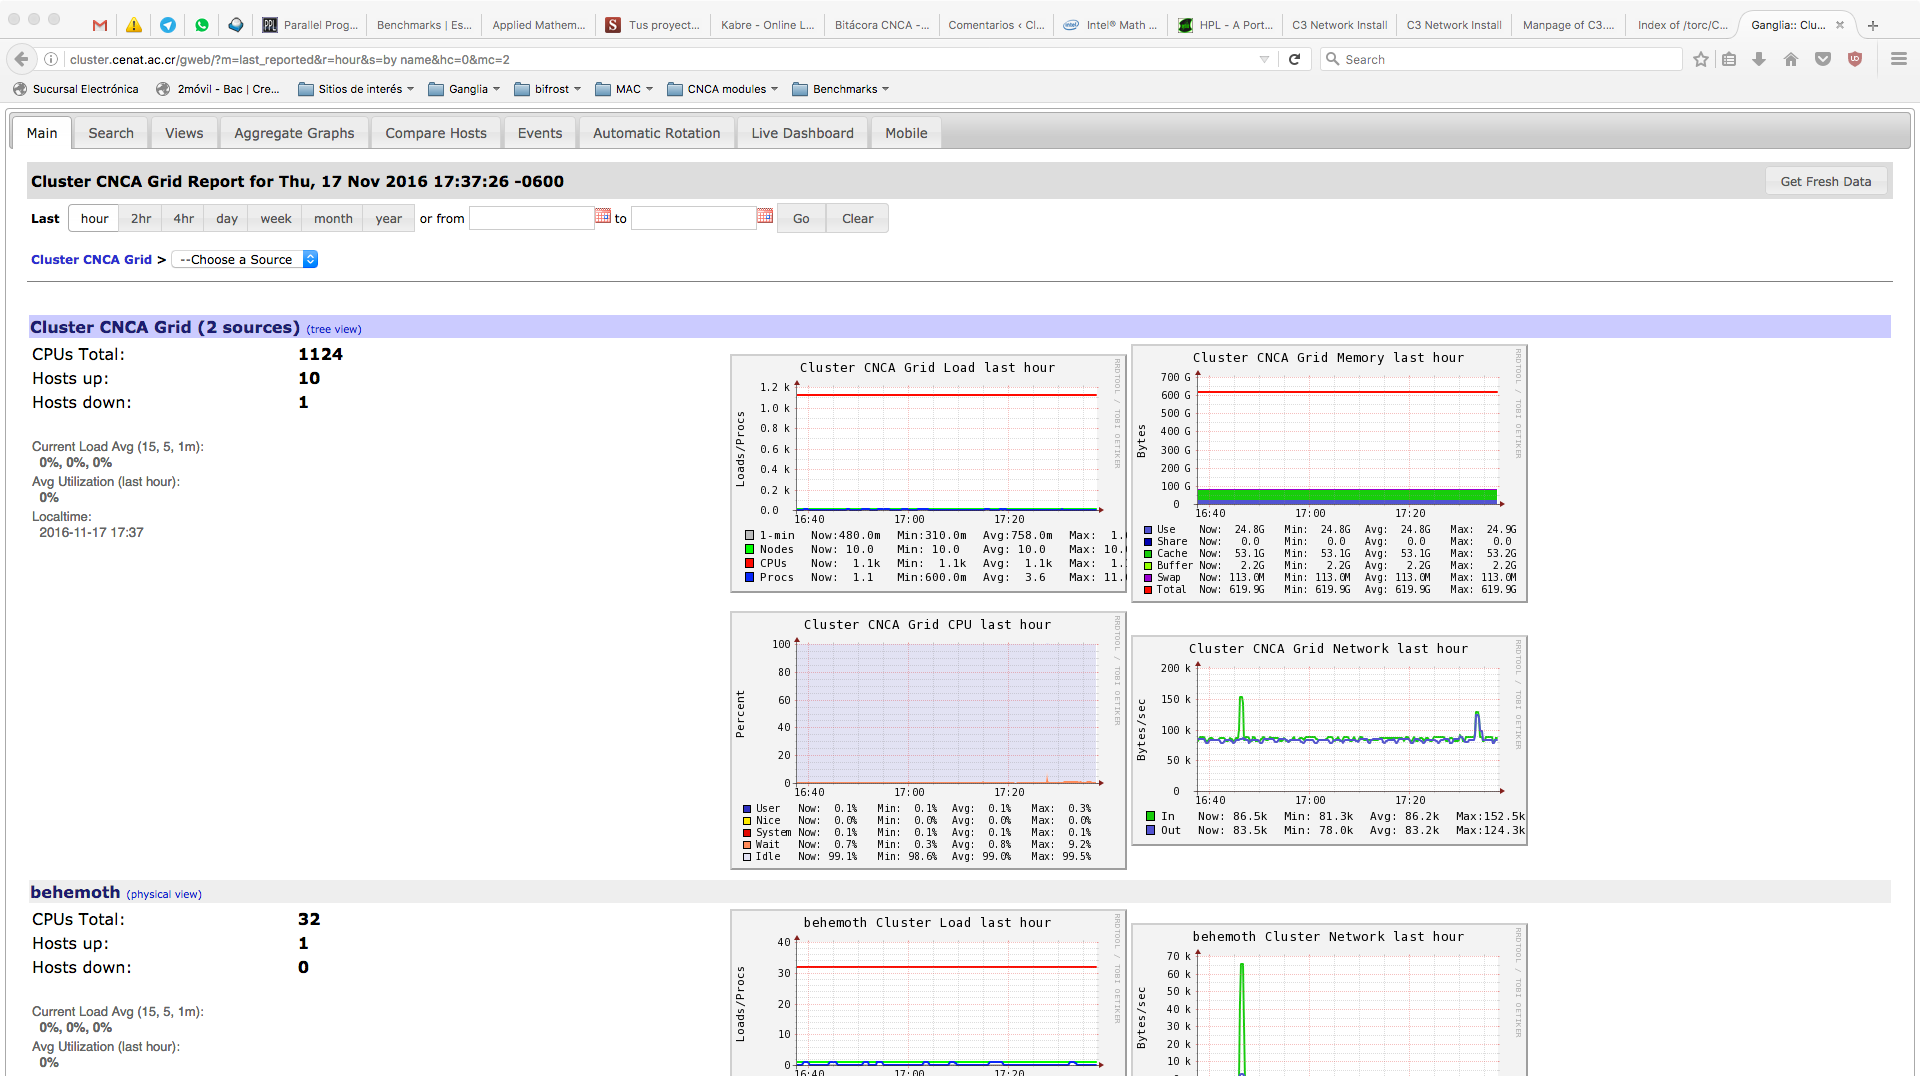
\includegraphics[width=0.7\textwidth]{ganglia_setting00.png}
\caption{Cliente de monitoreo web Ganglia para recursos computacionales del clúster.}
\label{fig:ganglia:00}
\end{figure}

\section{OpenIPMI}

IPMI (Intelligent Platform Management Interface) consiste en una serie de herramientas para el monitoreo y mantenimiento de sistemas computacionales de manera rápida, sencilla y centralizada \cite{ipmisupermicro}. Esta plataforma permite aprovechar la disponibilidad de distintos sensores para monitorear el equipo, particularmente a nivel de temperatura, así como realizar mantenimiento a nivel de BIOS, entre otras ventajas. Existen versiones implementadas sobre un cliente web para facilitar su uso remoto, así como versiones más básicas pero potentes a partir de CLI. La implementación que se instalará en el clúster es OpenIPMI \cite{openipmi}. Esta versión se encuentra ya disponible en los repositorios de CentOS, por l que su instalación es tan simple como hacer lo siguiente:

\begin{lstlisting}
yum -y install OpenIPMI OpenIPMI-devel OpenIPMI-libs OpenIPMI-modalias OpenIPMI-perl OpenIPMI-python
\end{lstlisting}

\subsection{Uso básico}


\section{Torque Monitor (PyMonSTor)}

PyMonSTor (Python Monitor Simple de Torque) es un programa que permite obtener una estadística de uso básica de los recursos del clúster a partir de los log files generados diariamente por el gestor de colas Torque. Esta información es de vital importancia para poder darle un mejor seguimiento al equipo y a los usuarios, de manera que las decisiones de adquisición de equipo nuevo, asignación de presupuesto, entre otros, tengan un mejor sustento técnico que los justifique.

La idea inicial es mostrar el aprovechamiento de los equipos en Service Units (Unidades de servicio), los cuales básicamente representan, para cada arquitectura disponible, la cantidad total de horas computacionales que puede proporcionar en un periodo de 24 horas. En este caso, las colas Zarate, correspondiente a los nodos phi, pueden proporcionar 96 SU por día, mientras que Cadejos proporciona 120 SU por día. Esto se obtiene siguiendo la ecuación \ref{SU}:

\begin{align}
SU_{arch} &= Nodes_{arch}*24 hours \label{SU}
\end{align}

\subsection{Estructura del log file de Torque}
Los archivos log se encuentran en el directorio /var/spool/torque/job\_logs en el nodo meta, y estos se general diariamente siguiendo la nomenclatura aaaammdd. El formato de estos archivos es una especie de xml no estándar, pues no cuentan con una llave raíz que contenga los demás subconjuntos, sino que contiene varias raíces, una para cada trabajo enviado al sistema de colas, y sigue la estructura mostrada a continuación:

\begin{lstlisting}
<Jobinfo>
	<Job_Id>10853.meta.cnca</Job_Id>
	<Job_Name>InfOliNTUA</Job_Name>
	<Job_Owner>djimenez@login-1.cnca</Job_Owner>
	<resources_used>
		<cput>1077</cput>
		<mem>60196kb</mem>
		<vmem>2043716kb</vmem>
		<walltime>130</walltime>
	</resources_used>
	<job_state>C</job_state>
	<queue>phi-debug</queue>
	<server>meta.cnca</server>
	<Checkpoint>u</Checkpoint>
	<ctime>1492441508</ctime>
	<Error_Path>login-1.cnca:/home/djimenez/InfOli-Comparison/scripts/InfOliNTUA.e10853</Error_Path>
	<exec_host>phi-a.cnca/0</exec_host>
	<exec_port>15003</exec_port>
	<Hold_Types>0</Hold_Types>
	<Join_Path>n</Join_Path>
	<Keep_Files>n</Keep_Files>
	<Mail_Points>a</Mail_Points>
	<mtime>1492441641</mtime>
	<Output_Path>login-1.cnca:/home/djimenez/InfOli-Comparison/scripts/InfOliNTUA.o10853</Output_Path>
	<Priority>0</Priority>
	<qtime>1492441508</qtime>
	<Rerunable>1</Rerunable>
	<Resource_List>
		<neednodes>phi-a.cnca</neednodes>
		<nodect>1</nodect>
		<nodes>phi-a.cnca</nodes>
		<procct>0</procct>
		<walltime>1800</walltime>
	</Resource_List>
	<session_id>49625</session_id>
	<substate>59</substate>
	<Variable_List>PBS_O_QUEUE=phi-debug,PBS_O_HOME=/home/djimenez,PBS_O_LOGNAME=djimenez,PBS_O_PATH=/opt/intel/compilers_and_libraries_2017.0.098/linux/bin/intel64:/opt/intel/compilers_and_libraries_2017.0.098/linux/mpi/intel64/bin:/opt/intel/debugger_2017/gdb/intel64_mic/bin:/opt/intel/compilers_and_libraries_2017.0.098/linux/mpi/intel64/bin:/opt/intel/compilers_and_libraries_2017.0.098/linux/bin/intel64:/opt/intel/compilers_and_libraries_2017.0.098/linux/mpi/intel64/bin:/opt/intel/debugger_2017/gdb/intel64_mic/bin:/usr/local/bin:/usr/bin:/usr/local/sbin:/usr/sbin:/home/djimenez/bin,PBS_O_MAIL=/var/spool/mail/djimenez,PBS_O_SHELL=/bin/bash,PBS_O_LANG=en_US.utf8,PBS_O_WORKDIR=/home/djimenez/InfOli-Comparison/scripts,PBS_O_HOST=login-1.cnca,PBS_O_SERVER=meta.cnca</Variable_List>
	<euser>djimenez</euser>
	<egroup>cluster</egroup>
	<hashname>10853.meta.cnca</hashname>
	<hop_count>1</hop_count>
	<queue_rank>94</queue_rank>
	<queue_type>E</queue_type>
	<etime>1492441508</etime>
	<exit_status>0</exit_status>
	<submit_args>-l nodes=phi-a.cnca InfOliNTUA.pbs</submit_args>
	<start_time>1492441509</start_time>
	<start_count>1</start_count>
	<fault_tolerant>0</fault_tolerant>
	<comp_time>1492441645</comp_time>
	<job_radix>0</job_radix>
	<total_runtime></total_runtime>
	<submit_host>login-1.cnca</submit_host>
</Jobinfo>

\end{lstlisting}

Algunos de los parámetros de tiempo mostrados están en formato Unix time, por lo que requieren de una adecuada conversión, para poder aprovecharlos. Posteriormente, las llaves de interés para el monitor son:

\begin{itemize}
\item[Job\_Owner]: Muestra el usuario que envió el trabajo a ejecutar en el sistema.
\item[resources\_used]: Despliega los recursos empleados
\item[walltime]: Indica el tiempo de uso de los recursos, en segundos.
\item[job\_state]: Indica si el trabajo se completó satisfactoriamente o si por el contrario ocurrió un error.
\item[queue]: Muestra la cola de trabajo particular utilizada para la ejecución.
\item[exec\_host]: Muestra los nodos que se utilizaron en el trabajo ejecutado.
\end{itemize}

Los parámetros de cada llave son de interés para efectos del monitor de recursos.

\subsection{Código fuente}
El programa como tal es un script escrito en python 3, el cual utiliza las siguientes bibliotecas:

\begin{itemize}
\item[untangle]: Biblioteca con funciones para parsear y manipular archivos xml.
\item[datetime]: Biblioteca para hacer operaciones con datos de fechas, incluyendo conversión de Unix time a fecha y hora estándar.
\item[matplotlib]: Biblioteca con funciones para la generación de gráficos a partir de estructuras de datos y archivos. Es compatible con diccionarios.
\item[re]: Es una biblioteca que agrega funciones adicionales para la manipulación de strings.
\end{itemize}

A continuación se muestra el script empleado. Este puede variar conforme se vaya mejorando y actualizando. Se generan gráficos con matplotlib en formato PDF, en los cuales se muestra la cantidad de SU por arquitectura y por usuario de cada día que se ejecute el script.

\lstinputlisting[language=Python]{pymonstor.py}


\clearpage